% Recursive fibre-tree / operator-traversal / residual-gradient diagram.
% Build: pdflatex fibre_tree.tex -> fibre_tree.pdf
\documentclass[border=6pt]{standalone}
\usepackage{tikz}
\usepackage{helvet}\renewcommand{\familydefault}{\sfdefault}
\usetikzlibrary{positioning,arrows.meta,fit,backgrounds,calc}
\begin{document}
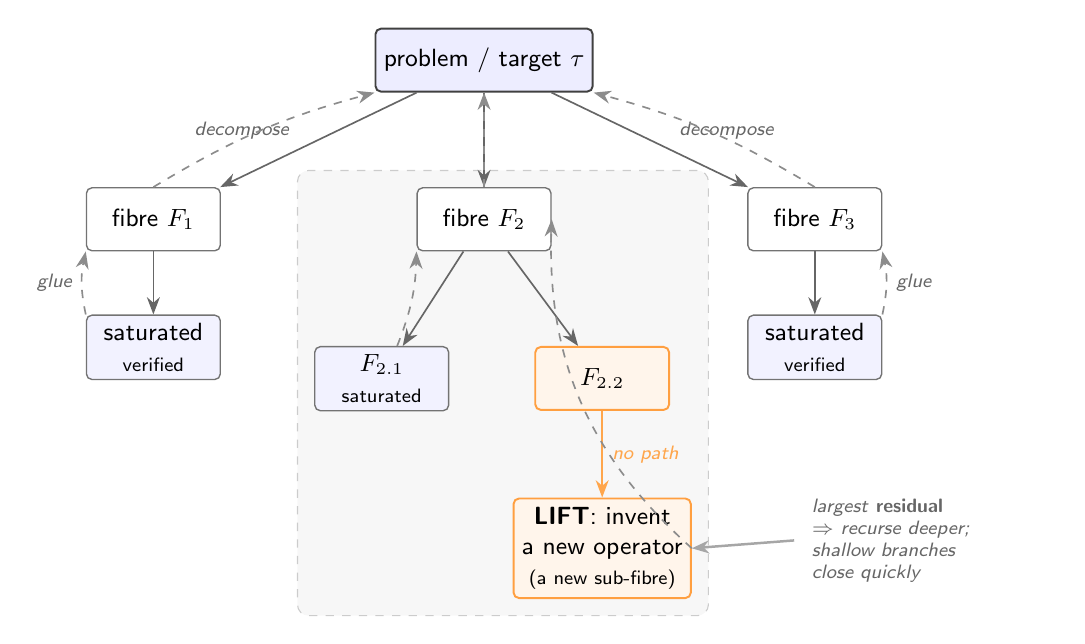
\begin{tikzpicture}[
  font=\small, >={Stealth[length=2.2mm]},
  fib/.style={rounded corners=2pt, draw=black!55, line width=0.5pt, align=center,
              inner sep=3pt, minimum height=8mm, minimum width=17mm, fill=white},
  goal/.style={fib, draw=black!75, fill=blue!7, line width=0.7pt},
  sat/.style={fib, fill=blue!5},
  invnode/.style={fib, draw=orange!75, fill=orange!8, line width=0.7pt},
  dec/.style={->, line width=0.6pt, draw=black!60},
  glue/.style={->, line width=0.6pt, draw=black!45, dashed},
  lbl/.style={font=\scriptsize\itshape, text=black!60},
  node distance=7mm and 8mm,
]
% root
\node[goal] (root) {problem / target $\tau$};
% level 1
\node[fib, below=12mm of root, xshift=-42mm] (f1) {fibre $F_1$};
\node[fib, below=12mm of root]              (f2) {fibre $F_2$};
\node[fib, below=12mm of root, xshift=42mm] (f3) {fibre $F_3$};
% level 2 under F2 (the high-residual branch, expanded deeper)
\node[sat, below=12mm of f2, xshift=-13mm] (f21) {$F_{2.1}$\\{\scriptsize saturated}};
\node[invnode, below=12mm of f2, xshift=15mm] (f22) {$F_{2.2}$};
% leaves resolved
\node[sat, below=8mm of f1] (f1r) {saturated\\{\scriptsize verified}};
\node[sat, below=8mm of f3] (f3r) {saturated\\{\scriptsize verified}};
% GROW: invent a new operator under F2.2
\node[invnode, below=11mm of f22, align=center] (lift) {\textbf{LIFT}: invent\\a new operator\\{\scriptsize (a new sub-fibre)}};

% decompose edges (down)
\draw[dec] (root) -- node[lbl,above left,pos=.6]{decompose} (f1);
\draw[dec] (root) -- (f2);
\draw[dec] (root) -- node[lbl,above right,pos=.6]{decompose} (f3);
\draw[dec] (f2) -- (f21);
\draw[dec] (f2) -- (f22);
\draw[dec] (f1) -- (f1r);
\draw[dec] (f3) -- (f3r);
\draw[dec, draw=orange!70] (f22) -- node[lbl,right,text=orange!70]{no path} (lift);

% glue edges (up, dashed)
\draw[glue] (f1r.north west) to[bend left=12] node[lbl,left]{glue} (f1.south west);
\draw[glue] (f21) to[bend right=10] (f2.south west);
\draw[glue] (lift.east) to[bend left=25] (f2.east);
\draw[glue] (f3r.north east) to[bend right=12] node[lbl,right]{glue} (f3.south east);
\draw[glue] (f1.north) to[bend left=8] (root.south west);
\draw[glue] (f2.north) -- (root.south);
\draw[glue] (f3.north) to[bend right=8] (root.south east);

% residual gradient (guides where to recurse deeper)
\begin{scope}[on background layer]
  \node[draw=black!20, dashed, rounded corners=4pt, fill=black!3,
        fit=(f2)(f21)(f22)(lift), inner sep=6pt] (hi) {};
\end{scope}
\node[lbl, align=left, text width=30mm, anchor=west] at ($(lift.east)+(14mm,1mm)$)
  {largest \textbf{residual}\\$\Rightarrow$ recurse deeper;\\shallow branches\\close quickly};
\draw[->, draw=black!35, line width=0.9pt] ($(lift.east)+(13mm,1mm)$) -- (lift.east);
\end{tikzpicture}
\end{document}
